\section{Отношения}

{\bfseries Определение.} {\slshape Упорядоченным набором}, или же {\slshape кортежем}, или же {\slshape отношением}, называется набор объектов, в котором так же определен порядок этих объектов.

Как обычно это совершенно чудовищное определение, которое не может считаться строгим математическим, но пока мы попробуем работать с ним, напирая на интуицию, а не научную строгость. Записывается упорядоченный набор как $(a, b, \ldots, z)$, где элементы $a$, $b$ и $z$ являются элементами некоторых определенных множеств.

Как более-менее практический пример можно рассмотреть базы данных. Чтобы не говорить слишком абстрактно, а рассмотреть более конкретную ситуацию, можно рассмотреть простую записную книжку мобильного телефона, которая тоже по сути является компьютерной базой данных.

Сама база данных представляет из себя множество записей, каждая из которых состоит из нескольких полей. Это можно представить как таблицу:

\begin{table}[h]
\begin{tabular}{lllll}
Фамилия & Имя & Телефон & ДР & Комментарий\\
Авраам & Линкольн & +1(270)... & 12.02.1802 & Президент\\
Бенито & Муссолини & +3(39)... & 29.07.1883 & Фашик\\
Владимир & Ленин & +7(499)... & 22.04.1870 & Свой мужик\\
Григорий & Распутин & +7(3459)... & 21.01.1869 & Есть чему завидовать\\
Джорджина & Байер & +6(64)... & 11.1957 & Транссексуал\\
... & ... & ... & ... & ...
\end{tabular}
\end{table}

Если предположить, что $F$ — множество фамилий, $N$ — множество имен, $P$ — множество телефонов, $D$ — множество дат календаря и $S$ — множество произвольных текстовых строк, то можно сказать, что данная таблица иллюстрирует множество упорядоченных наборов следующего вида:

$\{(f, n, p, b, c)|f\in F, n \in N, p \in P, b \in D, c \in S\}$

(Строго говоря с точки зрения логики правильнее было бы писать не символ запятой справа в предикате, а символ $\wedge$, но чаще в случаях, подобных нашему, употребляется именно запятая в силу большей наглядности и удобства — означает она при этом логическое И).

Практически вся теория баз данных построена на самом деле на теории множеств в рамках того, что я уже рассказал, и декартова произведения, о котором речь пойдет ниже. База данных — это множество, элементами которого являются упорядоченные наборы. Команды работы с базой данных — это операции, задающие предикаты и операции над множествами. Я не могу позволить себе углубляться сейчас в алгебру реляционных баз данных и синтаксис языка SQL, но вообще рекомендую всем читателям с этими вещами ознакомиться — будет небесполезно, а заодно увидите кучу примеров тому, о чем я сейчас говорю.

Здесь стоит еще сделать такое наблюдение по терминологии. Чаще всего термин кортеж применяется именно в теории баз данных, термин отношение применяется чаще всего в случае упорядоченных пар, в которых оба элемента принадлежат одному и тому же множеству $\{(x, y)|x\in A, y\in A\}$, а термин упорядоченный набор используется в остальных случаях. Здесь нет строгого формального разграничения, это просто сложившаяся практика, которая однако может часто нарушаться и в этом нет ничего преступного.

{\bfseries Определение.} {\slshape Декартовым}, или {\slshape прямым}, {\slshape произведением} множеств $A$ и $B$ называется множество $A\times B = \{(a, b)|a\in A, b\in B\}$.

Говоря человеческим языком, $A\times B$ — это множество всех возможных упорядоченных пар $(a, b)$, таких что $a\in A$ и $b \in B$.

{\bfseries Пример.} Пусть $A = \{0, 1\}$, а $B = \{a, b, c\}$. Тогда $A\times B = \{(0, a), (0, b), (0, c), (1, a), (1, b), (1, c)\}$.

Кое-какую интуицию относительно декартова произведения вероятно поможет развить иллюстрация в виде таблицы. Столбцы в ней отводятся для элементов одного множества, строки — для другого множества, а на пересечении стоит их декартово произведение:

$\begin{array}{c|ccc}\times & a&b&c\\ \hline 0 & (0,a) & (0, b) & (0, c) \\ 1 & (1, a)& (1, b) &(1, c)\end{array}$

{\bfseries Пример.} Часто с помощью декартова произведения можно описывать какие-то физические понятия. Пусть $A$ — множество мастей (червы, буби, крести, трефы), а $B$ — множество достоинств (6, 7, 8, ..., король, туз). Тогда $A \times B$ — множество игральных карт в колоде.

{\bfseries Упражнение.} Покажите, что в общем случае $A\times B \not = B \times A$. В каких частных случаях все же $A\times B = B \times A$?

Легко заметить, что $(A\times B)\times C \not= A\times (B \times C)$, поскольку в случае множества до знака равенства будут получаться пары вида $((a, b), c)$, а для множества справа от знака равенства будут пары $(a, (b, c))$. Однако как и раньше удобно считать, что произведение $A\times B\times C$ без скобок дает нам упорядоченные тройки $(a, b, c)$ так же без каких-либо специальных группировок. Для удобства часто, впрочем, считают, что и при наличии скобок декартово произведение дает обычные упорядоченные наборы: $(A\times B)\times C = \{(a, b, c)|a\in A, b\in B, c\in C\}$.

Каждое отношение таким образом является подмножеством декартова произведения $\rho \subset X\times X$ — в этом параграфе нас будут интересовать как раз такие отношения. Часто для удобства применяется так же следующая запись: если $(x, y) \in \rho$, то пишут $x\rho y$. Из последующего текста будет видно почему это удобно.

{\bfseries Пример.} Пусть $S$ — множество высказываний. Тогда любая логическая операция задает отношение на этом множестве. В простейшем случае, если рассматривать только одно истинное и ложное высказывание $S = \{0, 1\}$, то $\vee = \{(1, 0), (0, 1), (1, 1)\}$, $\leftrightarrow = \{(0, 0), (1, 1)\}$ и так далее. По аналогии любому предикату на множествах можно сопоставить в соответствие некоторое отношение (возможно, не из двух элементов).

{\bfseries Определение.} Отношение называется {\slshape рефлексивным}, если для любого $x$ выполняется $x\rho x$.

{\bfseries Определение.} Отношение называется {\slshape антирефлексивным}, если для любого $x$ отношение $x\rho x$ не имеет места быть.

{\bfseries Определение.} Отношение называется {\slshape транзитивным}, если для любых $x$, $y$ и $z$ из того, что $x\rho y$ и $y \rho z$ следует, что $x\rho z$.

{\bfseries Определение.} Отношение называется {\slshape симметричным}, если из того, что $x\rho y$ следует $y\rho x$.

{\bfseries Определение.} Отношение называется {\slshape антисимметричным}, если из того, что $x \rho y$ и $y \rho x$ следует, что $x = y$.

Можно привести и больше возможных общих свойств отношений, но для наших нужд достаточно и того что я уже привел.

{\bfseries Упражнение.} Запишите эти свойства на языке логики.

{\bfseries Упражнение}. Приведите пример нетранзитивного отношения на множестве $\{0, 1\}$.

{\bfseries Определение.} Отношение называется {\slshape отношением эквивалентности}, если оно рефлексивно, транзитивно и симметрично.

Отношение эквивалентности часто обозначается символами $=$, $\approx$, $\sim$ и подобными (хотя есть и другие обозначения, которые мы будем по ситуации использовать). Если на множестве задано несколько отношений эквивалентности, то символьное обозначение отношения часто указывается справа внизу от знака эквивалентности: $\approx_R$.

{\bfseries Упражнение.} Пусть $S$ — множество учеников средней школы №469. Отношение $x\approx_Y y$ означает, что ученики $x$ и $y$ заканчивают школу в одном году, отношение $x \approx_C y$ означает, что они учатся в одном классе, $x \sim y$ что имеют одинаковую успеваемость. Проверьте, что все заданные отношения — это отношения эквивалентности (для этого необходимо проверить, что они рефлексивны, транзитивны и симметричны).

Следующие три упражнения уже посложнее, и их начинающие могут пропустить.

{\bfseries Упражнение.} Пусть $S$ — некоторое множество, а $P$ — множество предикатов, определенных на этом множестве. Пусть нам задано такое отношение, что $p \approx q$ тогда и только тогда, когда $p$ и $q$ определяют одинаковые подмножества $S$. Докажите, что это отношение эквивалентности.

{\bfseries Упражнение.} Пусть нам задано множество логических формул, все с одинаковым числом параметров. Отношение $f=g$ определено для функций, которые на одинаковых значениях параметров принимают одинаковые значения истинности. Докажите, что это отношение эквивалентности.

{\bfseries Упражнение.} Пусть нам задана некоторая теория. Докажите, что семантическая эквивалентность формул является отношением эквивалентности. (Напомню, что формулы $\phi$ и $\psi$ семантически эквивалентны, если в любой модели теории $\psi\leftrightarrow\phi$).

Примеры, приведенные в упражнении, демонстрируют основную идею отношения эквивалентности: это набор пар, которые имеют какие-то общие характеристики, которые и отражают отношение. Причем мыслить об отношении как о парах элементов чаще всего не удобно с интуитивной точки зрения — удобнее мыслить об отношении эквивалентности именно как о наличии какого-то общего свойства.

{\bfseries Определение.} Пусть дано множество $A$ и на нем задано отношение эквивалентности $\sim$. Множество всех элементов $x$, для которых $a\sim x$ называется {\slshape классом эквивалентности} элемента $a$ и обозначается как $[a]$.

{\bfseries Теорема.} Для любых элементов $a, b \in A$ классы эквивалентности $[a]$ и $[b]$ либо совпадают, либо не пересекаются.

{\bfseries Доказательство.} Проведем доказательство от противного и предположим, что теорема неверна. Пусть классы эквивалентности $[a]$ и $[b]$ пересекаются, но не совпадают. Тогда найдется элемент $x$, принадлежащий сразу обоим классам эквивалентности, и элемент $b' \in [b]$, такой что $b' \not\in [a]$. Для него однако верно, что $b' \sim x$, но поскольку $x \in [a]$ и $x\sim a$, то в силу транзитивности $b' \sim a$ и соответственно $b' \in [a]$. Полученное противоречие говорит, что наше предположение «от противного» было не верно, и значит теорема верна. \qed

Это доказательство на первый взгляд может показаться странным и непонятным — вспомните тогда свойства импликации $(a\rightarrow b) \leftrightarrow (\neg b \rightarrow \neg a)$ и как она связана с выводимостью (см. §1.6).

Смыслом теоремы является тот факт, что каждое множество с заданным на нем отношением эквивалентности можно разбить на непересекающиеся классы эквивалентности.

{\bfseries Пример.} Пусть опять $S$ — множество учеников школы №469. Всех учеников можно сгруппировать по классам, по успеваемости или по году окончания школы. Пусть $A$ — множество двоечников, $B$ — троечников, $C$ — хорошистов и $D$ — отличников. Очевидно, что эти множества не пересекаются и $S = A\cup B\cup C\cup D$, причем любые два ученика из одного и того же множества находятся в отношении $\sim$ («имеют одинаковую успеваемость») друг с другом, а ученики из разных множеств в этом отношении не находятся.

{\bfseries Определение.} Процесс разбиения множества на классы эквивалентности называется {\slshape факторизацией}, а само множество классов эквивалентности называется {\slshape фактор-множеством}. Если $\rho$ — отношение эквивалетности на $A$, то фактормножество $A$ по $\rho$ обозначается как $A/\rho$.

{\bfseries Пример.} Продолжая пример с успеваемостью, можно записать, что $S/\sim = \{A, B, C, D\}$.

Обратите внимание в какую сторону рисуется черта фактормножества и не путайте ее с разностью множеств. $A\setminus B$ — разность, а $A/\rho$ — факторизация.

Интуитивно таким образом можно рассматривать факторизацию как разбиение множества на подмножества в соответствии с некоторым отношением («фактором»). Обратное кстати тоже верно — если множество разбито на непересекающиеся подмножества, то по ним можно задать отношение эквивалентности.

{\bfseries Упражнение.} Пусть $A = \{a, b, c, d\}$ разбито на подмножества $\{a, b\}$ и $\{c, d\}$. Запишите по этому разбиению отношение эквивалентности $\rho$ как множество упорядоченных пар (начинается эта запись как $\rho = \{(a, a), (a, b), \ldots\}$).

Перейдем теперь ко второму не менее важному отношению, которое мы сравнительно часто будем использовать.

{\bfseries Определение.} Отношение называется {\slshape отношением частичного порядка} (или {\slshape отношением нестрогого частичного порядка}), если оно рефлексивно, транзитивно и антисимметрично.

{\bfseries Определение.} Отношение называется {\slshape отношением строгого частичного порядка}, если оно антирефлексивно, транзитивно и антисимметрично.

Отношение частичного порядка удобно обозначать как $\le$. Отношение строго частичного порядка как $<$. Если $a \le b$ и $a \not= b$, то $a<b$. Если $b \le a$, то можно писать $a \ge b$ или $a > b$, если $a\not= b$. Легко видеть, что отношения частичного и строгого частичного порядка — это фактически одного и то же. Различаются они лишь тем, находится ли каждый элемент в отношении с самим собой (то есть можем ли мы записать отношение $x\le x$). В теории в основном используется отношение частичного порядка, в конкретных задачах часто может оказаться удобным и то и другое. Хотя погоды это разграничение не делает: если у нас есть строгий порядок, то его всегда можно сделать не строгим, дополнив парами $x\le x$, и наоборот нестрогий порядок можно сделать строгим, выкинув такие пары.

{\bfseries Упражнение.} Докажите, что если элементами множества являются множества (например, это булеан), то отношение $\subset$ является отношением частичного порядка.

{\bfseries Упражнение.} Докажите, что отношение «является предком» на множестве людей является строгим частичным порядком.

{\bfseries  Упражнение.} Докажите, что отношение «не ниже чем» на множестве всех людей образует нестрогий частичный порядок, а отношение «выше чем» строгий частичный порядок.

{\bfseries Упражнение.} Покажите, что отношение «является родителем» не является отношением частичного порядка.

{\bfseries Упражнение.} Покажите, что на множестве картонных коробок отношение «влезает в» является отношением строгого частичного порядка.

{\bfseries Упражнение.} Рассмотрим множество всех логических функций с одинаковым числом параметров. Определим на них отношение следующим образом: $f\le g$ тогда и только тогда, когда на одинаковых наборах параметров либо эти функции принимают одинаковое значение, либо $f=0$, а $g=1$. Докажите, что отношение частичного порядка. Как оно соотносится с порядком на булеане множества?

{\bfseries Пример.} В микроэкономике рассматриваются отношения предпочтений, задаваемые на множествах альтернатив (читай товаров). Считается, что потребители могут сравнивать альтернативы по степени предпочтительности и данное отношение является как раз отношением частичного порядка. (Психологи однако доказывают, что предпочтения людей не являются рациональными и таким образом не образуют частичный порядок на множестве товаров).

Отношение частичного порядка удобно представлять в виде диаграмм. Например, так будет выглядеть диаграмма для булеана множества $\{x, y, z\}$:

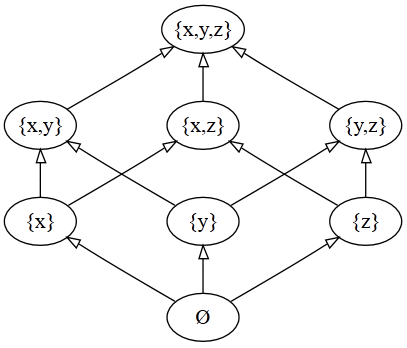
\includegraphics{hasse1.png}

(Картинка из Википедии, свободной энциклопедии, потому что сам не умею пока такие рисовать; LibreOffice Draw не справляется с задачей).

Здесь стрелка обозначает отношение «является подмножеством». Элементы, располагающиеся выше, оказываются «больше» элементов, располагающихся внизу, если между ними есть путь из стрелок. Если на диаграмме есть стрелка $a\to b$ и стрелка $b\to c$, то по транзитивности должна быть и стрелка $a\to c$, которая не указывается, чтобы не загромождать картинку.

Отношение частичного порядка таким образом упорядочивает элементы множества. Существенно, однако, что если задан частичный порядок, то совершенно не факт, что удастся сравнить произвольные два объекта. Как видно из диаграммы выше, элементы $\{x, y\}$ и $\{z\}$ не сравнимы между собой. Точно так же для любых двух людей не обязательно кто-то один из них должен быть предком другого, и в этом смысле не сравнимыми являются брат и сестра.

{\bfseries Определение.} {\slshape Линейным порядком} называется отношение частичного порядка, относительно которого сравнимы любые два элемента множества.

{\bfseries Пример.} Отношение «не ниже чем» является линейным порядком на множестве людей.

{\bfseries Определение.} {\slshape Максимальным элементом} называется такой элемент, что не существует элемента, большего него.

{\bfseries Определение.} {\slshape Наибольшим элементом} называется такой элемент, что он больше любого другого элемента.

{\bfseries Пример.} На множестве коробок максимальным элементом будет коробка, которая не может влезть ни в какую другую коробку. Наибольшим элементом будет коробка, в которую может поместиться любая другая коробка.

В полной аналогии можно ввести понятия {\slshape минимального} и {\slshape наименьшего элемента}, но мы не будем на это отвлекаться, так там вся теория совершенно аналогична.

Очевидно, что если множество обладает наибольшим элементом, то он же будет и единственным максимальным элементом. Однако же максимальных элементов может быть несколько, и наибольшего элемента в этом случае не будет, как в случае следующей диаграммы:

\begin{picture}(100,60)
\put(0,0){a}
\put(40,0){b}
\put(20,50){e}
\put(22,45){\line(-1,-2){18}}
\put(22,45){\line(1,-2){18}}
\put(80,0){c}
\put(120,0){d}
\put(100,50){f}
\put(102,45){\line(-1,-2){18}}
\put(102,45){\line(1,-2){18}}
\end{picture}

На приведенной диаграмме два максимальных элемента: $e$ и $f$. Наибольшего элемента нет. На следующей же диаграмме уже имеется один наибольший элемент $g$, он же является и максимальным:

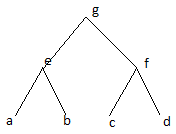
\includegraphics{hielement.png}

(Я правда надеюсь, что мне кто-нибудь из читателей поможет с иллюстрациями).

В обоих этих примерах порядки не являлись линейными. В случае же линейного порядка, очевидно, что понятия максимального и наибольшего элемента совпадают.

{\bfseries Определение.} {\slshape Верхней гранью} подмножества $S\subset U$ называется такой элемент $x\in U$, что для любого элемента $s\in S$ выполняется $s \le x$.

{\bfseries Определение.} {\slshape Нижней гранью} подмножества $S\subset U$ называется такой элемент $x\in U$, что для любого элемента $s\in S$ выполняется $s \ge x$.

Если $x$ — верхняя грань подмножества $S$, то любой элемент больший $x$ так же будет являться верхней гранью $S$. Таким образом, верхние грани сами по себе образуют множество (аналогично с нижними) и есть смысл ввести следующие определения:

{\bfseries Определение.} {\slshape Наименьшей}, или {\slshape точной}, {\slshape верхней гранью}, называется наименьшая из верхних граней. Обозначается она как $\sup S$.

{\bfseries Определение.} {\slshape Наибольшей}, или {\slshape точной}, {\slshape нижней гранью}, называется наибольшая из нижних граней. Обозначается она как $\inf S$.

(С этого места начинаются абстракции, которые начинающему читателю вероятно и не являются необходимыми — если будет не понятно о чем речь, можно смело пропускать. Если однако разобраться с материалом, то это будет хорошим упражнением для ума.)

Если подмножество $S$ состоит лишь из двух элементов, то операции «точных граней» можно рассматривать как арифметические операции над этими элементами. В этом случае используется запись $\sup\{a, b\} = a\vee b$ и $\inf\{a, b\} = a\wedge b$.

{\bfseries Упражнение.} Докажите, что на булеане относительно порядка, образованного включением множеств, $A\wedge B = A\cap B$ и $A\vee B = A \cup B$ и они обладают соответственно всеми свойствами логического И и логического ИЛИ.

Сформулированное в упражнении утверждение в общем случае неверно, если рассматривать произвольный частичный порядок. Во-первых, могут не выполняться сами свойства логических операций, а во-вторых самих точных граней может и не быть. Поэтому вводятся следующие определения:

{\bfseries Определение.} {\slshape Решёткой} называется частично упорядоченное множество, у которого для любого двухэлементного подмножества существуют точные верхние и нижние грани.

{\bfseries Определение.} {\slshape Дистрибутивной решёткой} называется решётка, для которой оказываются верны свойства дистрибутивности операций $\wedge$ и $\vee$ (см §1.1, теорема 1).

{\bfseries Упражнение.} Докажите, что решётка, изображенная на диаграмме ниже, не является дистрибутивной:

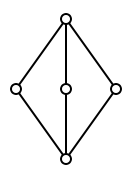
\includegraphics{lattice.png}

Дистрибутивные решетки уже практически дублируют законы логики, которым была посвящена первая глава. Не достает только $1$ и $0$. Следующие определения исправляют ситуацию:

{\bfseries Определение.} Решетка называется ограниченной, если в ней существуют наибольший и наименьший элементы, обозначаемые соответственно как $0$ и $1$.

{\bfseries Упражнение.} Если решетка имеет минимальный или максимальный элементы, то они будут единственны и будут являться наименьшим и наибольшим элементами. Докажите это.

{\bfseries Определение.} {\slshape Дополнением} элемента $x$ ограниченной решетки такой элемент $y$, что $x\wedge y = 0$ и $x \vee y = 1$. Дополение $x$ обозначается как $\neg x$.

{\bfseries Определение.} Если в решетке каждый элемент обладает дополнением, то такая решетка называется {\slshape решеткой с дополнением}.

{\bfseries Определение.} {\slshape Булевой алгеброй} называется дистрибутивная решетка, обладающая наименьшим и наибольшим элементами (обозначаемыми соответственно $0$ и $1$).

{\bfseries Пример.} Если рассмотреть двухэлементное множество $\{0, 1\}$ и определить на нем порядок $0 < 1$, то мы получим в точности классическую логику, которую рассматривали в первой главе, которая как теперь видно является разновидностью булевой алгебры.

{\bfseries Пример.} Булеан любого множества $A$ задает булеву алгебру относительно включения множеств, где наибольшим элементом является само множество $A$, а наименьшим пустое множество.

{\bfseries Упражнение.} Для булевых алгебр справедливы все законы логики, которые мы приводили в теореме 1.1. Докажите это.

Если у нас есть два частично упорядоченных множества $A$ и $B$, то на их декартовом произведении можно задать частичный порядок несколькими способами:

{\bfseries Определение.} {\slshape Лексигографическим порядком} на $A\times B$ называется порядок, при котором $(a, b) \le (a', b')$ либо когда $a < a'$, либо когда $a=a'$ и $b\le b'$.

{\bfseries Определение.} {\slshape Естественным порядком} на $A\times B$ называется порядок, при котором $(a, b) \le (a', b')$ тогда и только тогда, когда одновременно $a \le a'$ и $b \le b'$.

Оба этих порядка естественно распространяются на декартово произведение любого количества множеств.

{\bfseries Упражнение.} Пусть $B = \{0, 1\}$ и на нем введен порядок $0 < 1$. Будем рассматривать множество $B\times B\times \ldots \times B$ (фактически упорядоченные наборы единиц и нулей) с естественным частичным порядком. Докажите, что такой частичный порядок задает булеву алгебру (кстати, как раз ту самую, которая повсеместно используется в программировании и называется там побитовыми логическими операциями).

{\bfseries Упражнение.} Докажите, что линейно-упорядоченное множество является дистрибутивной решеткой, и соответственно при наличии наименьшего и наибольшего элемента является булевой алгеброй.

{\bfseries Упражнение.} Является ли булевой алгеброй множество $B\times B \times \ldots \times B$, введенное выше, относительно лексикографического порядка?

{\bfseries Упражнение.} Пусть теперь $B$ — некоторая произвольная булева алгебра. Является ли булевой алгеброй $B\times B \times \ldots \times B$ относительно лексикографического порядка? А относительно естественного порядка?
